



\documentclass[12pt]{report}

% for navigation within the generated pdf
\usepackage{hyperref}
% for abbreviations
\usepackage{acro}
% for code snippets
\usepackage{listings}
% to frame code listings nicely in a box
\usepackage{framed}
% for color utilities
\usepackage{xcolor}
% for figs
\usepackage{graphicx}
% for new fonts
\usepackage{courier}
% avoid showing "Chapter" text
\usepackage{titlesec}


\DeclareAcronym{sihft}{
  short=SIHFT,
  long=Software Implemented Hardware Fault Tolerance,
}

% make sure no indentation done for new paragraphs
\setlength\parindent{0pt}


% title content
\date{\today}
\title{
\textbf{COMPAS-FT-RISCV} \\
\large Compiler Assisted Fault Tolerance for RISCV Architectures \\
\small Version 1.0.0
}
\author{
ESL Group, Chair of Electronic Design Automation \\
Department of Electrical and Computer Engineering \\
Technical University of Munich
}

% avoid showing meaningless "Chapter" for manual content
\titleformat{\chapter}[display]
  {\normalfont\huge\bfseries}{}{0pt}{\Huge}
\titlespacing*{\chapter}
  {0pt}{10pt}{40pt}

% disable hyperref colors on links in generated pdf
% \hypersetup{
%   colorlinks=true, linkcolor=black, anchorcolor=black, citecolor=black,
%   filecolor=black, menucolor=black, runcolor=black, urlcolor=black]
% }
\hypersetup{
  colorlinks=true, linkcolor=black, anchorcolor=black, citecolor=black,
  filecolor=black, menucolor=black, runcolor=black, urlcolor=black
}

\begin{document}

\maketitle

\tableofcontents
\listoffigures

\newpage
\printacronyms

\chapter{User Manual}

\section{Overview}
COMPAS-FT-RISCV compiler was developed as part of the research work conducted in SAFE4I project. SAFE4I is funded by
the BMBF Ministry (Germany's Federal Ministry of Education and Research) under project grant 01IS17032. The authors
are responsible for the content of this document. \\

Compiler transformations to build soft error resilience into embedded software are highly attractive owing to their
superior error detection as well as automation properties. Before starting this work, we experienced a tooling
gap with in the RISC-V eco-system for ensuring functional safety for embedded firmware. This work aims to fill this gap
by providing a library of LLVM passes (C++ modules) that can be integrated in a modern LLVM codebase.
The resulting compiler is then able to provide various state-of-the-art
\textit{Software Implemented Hardware Fault Tolerance} (\ac{sihft}) transformations on a given C/C++ project. \\

Specifically, we have implemented the following \ac{sihft} methods:
\begin{itemize}
 \item{EDDI \cite{eddi} for data-flow protection}
 \item{SWIFT \cite{swift} for data-flow protection}
 \item{NZDC \cite{nzdc} for data-flow protection}
 \item{NEMESIS \cite{nemesis} for conditional branch protection}
 \item{CFCSS \cite{cfcss} for control flow protection}
 \item{RASM \cite{rasm} for control flow protection}
 \item{REPAIR \cite{repair} for combined data-flow and control-flow protection}
\end{itemize}

This document serves to be the user manual for the developed compiler. We now provide instructions on how to setup the
LLVM compiler in order to use the implemented \ac{sihft} transformations.

% installation guide section
\newpage


\chapter{Installation Guide}
\label{ch:Install}

In this chapter, we provide instructions on how to integrate our developed \ac{sihft} passes within the LLVM codebase.
This allows us later to carry out various \ac{sihft} transformations during LLVM backend compilation in generating
RISCV code.

\section{Development System}
The instructions given in this user manual are expected to work on any Linux machine. Specifically, we have prepared
this manual while developing on a freshly installed Ubuntu 20.04 PC.

\subsection{Ubuntu Packages}
Following packages are needed to be installed:

\begin{itemize}
 \item{C++ compiler like gcc/g++}
 \item{CMake}
 \item{git}
\end{itemize}

Following commands can be used to install them:

\begin{lstlisting}[language=bash, frame=single, basicstyle=\small\ttfamily]
$ sudo apt install build-essential cmake git
  \end{lstlisting}

\section{Build LLVM Project}
\label{sec:build-llvm}
The LLVM Project has to be compiled from source. We recommend downloading version 13.0.0 from LLVM Releases webpage:
\\\\
\url{https://releases.llvm.org/} \\

With the downloaded source package extracted, execute the following commands on your bash shell to build
llvm project from source:

\begin{framed}
 \begin{lstlisting}[language=bash, basicstyle=\small\ttfamily]
$ cd <llvm_src_folder>
$ mkdir build
$ cd build
$ cmake -DCMAKE_BUILD_TYPE=Release
        -DCMAKE_INSTALL_PREFIX=<install_location>
        -DCMAKE_CXX_STANDARD=17
        -DLLVM_ENABLE_PROJECTS=clang
        -DLLVM_TARGETS_TO_BUILD=RISCV
        -DLLVM_ENABLE_ASSERTIONS=ON 
        ../llvm
$ make
  \end{lstlisting}
\end{framed}

\textit{NOTE: The paths mentioned above as $<$...$>$ need to be adapted as per your filesystem.} \\

In the \texttt{<build>/bin} directory, we should now see llvm executable programs and utilities like
\texttt{clang}, \texttt{llc} etc. Run them to make sure they are built fine. For example, we can run the
static compiler \texttt{llc} to make sure that RISCV targets are supported as shown in Fig.~\ref{fig:llc}. \\

\begin{figure}[tb]
 \centering
 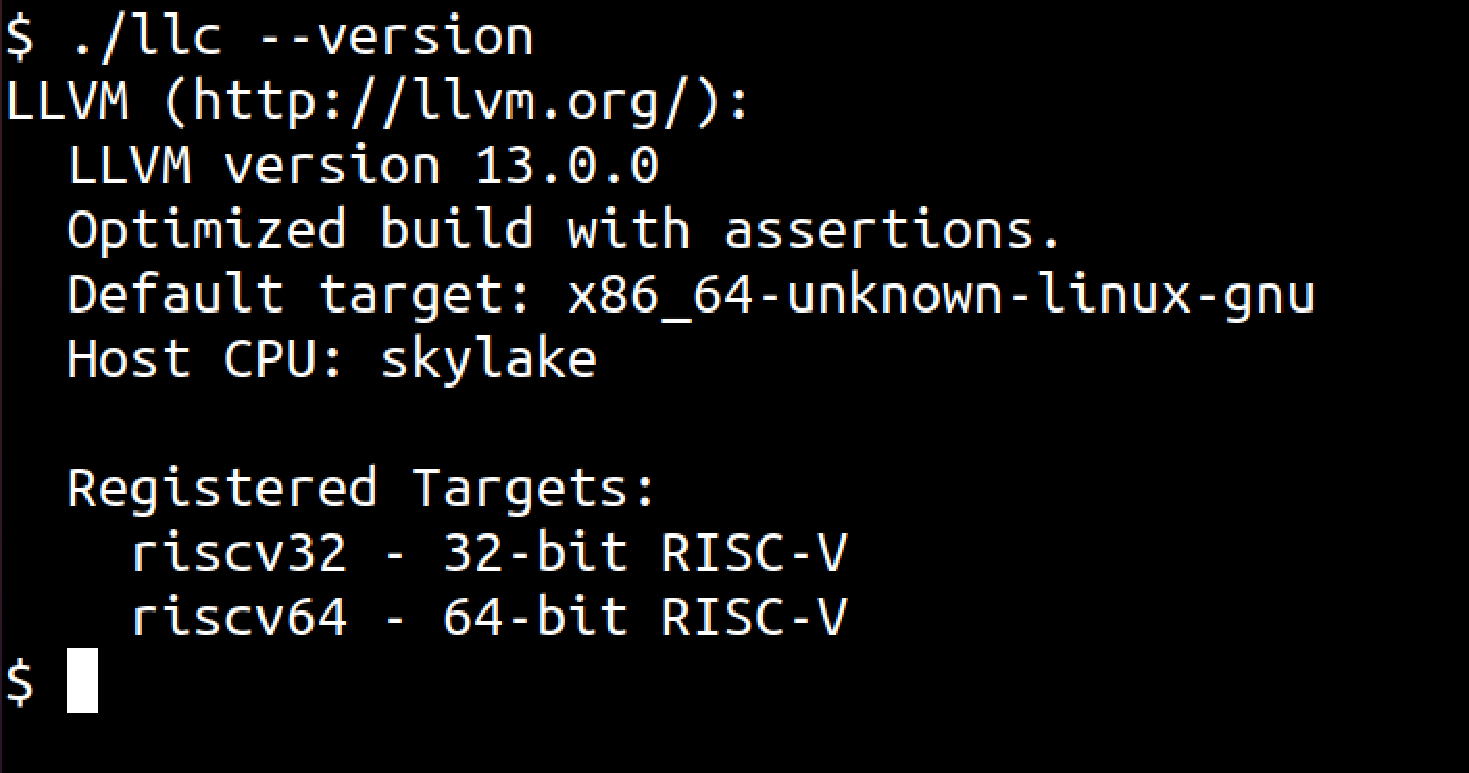
\includegraphics[width=\linewidth]{figs/llc.pdf}
 \caption{Expected output of sanely built \texttt{llc}}
 \label{fig:llc}
\end{figure}

\textit{NOTE: Make using parallel jobs (\texttt{make -jN}) would help significantly to reduce the compile time
 for a large codebase like LLVM. However, we encourage to do this on a server. For systems having lesser memory, make
 with parallel jobs has to be used cautiously, as the command could fail due to memory exhaustion issues.}

\newpage
\section{Integrate \ac{sihft} Passes}
The first step is to clone our open-source \texttt{compas-ft-riscv} repository within the LLVM source tree. Afterwards,
the patch is applied on RISCV backend in order to register the new transformation passes. Finally, the LLVM project
is rebuilt.

The corresponding shell commands are shown below. Here \texttt{<path\_to\_patch>} variable should be substituted
with a compatible patch file. For this, we provide various patches in our passes repository.
Each patch is compatible with a specific llvm project source tree.
In case this tutorial is followed to build llvm project using Sec.~\ref{sec:build-llvm},
the corresponding patch is to be found at:\\\\
\texttt{compas-ft-riscv/patches/llvm13.0.0\_src.patch}

\begin{framed}
 \begin{lstlisting}[language=bash, basicstyle=\small\ttfamily]
$ cd <llvm_src_folder>/llvm/lib/Target/RISCV/
$ git clone https://github.com/tum-ei-eda/compas-ft-riscv
$ cd <llvm_src_folder>
$ patch -s -p0 < <path_to_patch>
$ cd build
$ make
$ make install
\end{lstlisting}
\end{framed}

Here, at the end we install the built llvm compiler infrastructure. Again make sure that the compiler is installed fine
by using Fig.~\ref{fig:llc}.


% user guide section
\newpage


\section{Usage Guide}

Various \ac{sihft} passes can be invoked via command line arguments to the LLVM static compiler \texttt{llc} program.
This chapter assumes that the LLVM compiler has been installed as per instructions in earlier sections.
We refer the installation location of this compiler to \texttt{<llvm\_install>} in rest of the chapter.

\subsection{\ac{sihft} Compilation}
Each source file (translation unit) in C/C++ project has to be first compiled to LLVM IR code using \texttt{clang}.
Following command can be used to generate human readable LLVM IR code representation of given C source file.
\begin{framed}
 \begin{lstlisting}[language=bash, basicstyle=\small\ttfamily]
$ <llvm_install>/bin/clang
    -emit-llvm -S <other options>
    main.c -o main.ll
  \end{lstlisting}
\end{framed}

The next step in the compilation is to pass the LLVM IR file to \texttt{llc} program:\\
\begin{lstlisting}[language=bash, basicstyle=\small\ttfamily, frame=single]
$ <llvm_install>/bin/llc
    <SIHFT options> <other options>
    main.ll -o main_hardened.s
\end{lstlisting}

\texttt{<SIHFT options>} refer to various \ac{sihft} transformations that we have developed. A brief overview of these
options is provided in Table~\ref{tab:sihft-options}.

\begin{table}[htb]
 \centering
 \caption{Supported \ac{sihft} options}
 \label{tab:sihft-options}

 \begin{tabular}{|l|l|}
  \hline
  \textbf{Option}                       & \textbf{Description}                                     \\
  \hline
  -NZDC=\textless foo, bar\textgreater  & apply NZDC transformation on \textit{foo,bar} functions  \\
  -RASM=\textless foo, bar\textgreater  & apply RASM transformation on \textit{foo,bar} functions  \\
  -CFCSS=\textless foo, bar\textgreater & apply CFCSS transformation on \textit{foo,bar} functions \\
  -FGS                                  & use fine-grain scheduling for NZDC code                  \\
  -REPAIR                               & use REPAIR transformation on NZDC code                   \\
  \hline
 \end{tabular}
\end{table}

The final step in code generation is to use \texttt{gcc} for RISCV architectures to assemble and link the
assembly code for a particular RISCV processor.

\subsubsection{Example}
For the sake of example, assume we want to protect the \texttt{crc} program from the MiBench suite. The
compiled program is to run on the RISCV spike simulator. The C project contains the following C files:

\begin{itemize}
 \item{crc.h: header for CRC library functions}
 \item{crc.c: source for CRC library functions}
 \item{main.c: contains the \texttt{main} program to invoke crc library functions}
\end{itemize}

Following commands are issued on bash shell to create the RISCV binary with
\begin{itemize}
 \item NZDC, RASM protection on \texttt{crcSlow} function
 \item RASM protection on \texttt{crcFast} function
 \item NZDC, CFCSS protection on \texttt{main} function
\end{itemize}

\begin{framed}
 \begin{lstlisting}[language=bash, basicstyle=\small\ttfamily]
$ cd <crc-project-source>

$ <clang> -emit-llvm -O2 -S --target=riscv64
    -march=rv64gc -mabi=lp64d
    -isystem <riscv64-gcc>/riscv64-unknown-elf/
    main.c -o main.ll
$ <clang> -emit-llvm -O2 -S --target=riscv64
    -march=rv64gc -mabi=lp64d
    -isystem <riscv64-gcc>/riscv64-unknown-elf/
    crc.c -o crc.ll

$ <llc> -O2 -march=riscv64 -mattr=+m,+a,+d,+c
    -NZDC=main -CFCSS=main
    main.ll -o main_hardened.s
$ <llc> -O2 -march=riscv64 -mattr=+m,+a,+d,+c
    -NZDC=crcSlow -RASM=crcSlow,crcFast
    crc.ll -o crc_hardened.s

$ <riscv64-gcc>/bin/riscv64-unknown-elf-gcc -O2
    -march=rv64gc -mabi=lp64d
    main_hardened.s crc_hardened.s -o crc_hardened.elf

$ spike pk crc_hardened.elf

\end{lstlisting}
\end{framed}

% \newpage
% \section{Configuration via TOML script}


% references
\bibliographystyle{apalike}
\bibliography{references}


\end{document}
